\documentclass[11pt,a4paper]{article}

\usepackage[margin=2cm]{geometry}
\usepackage[compact]{titlesec}
\usepackage[T1]{fontenc}
\usepackage{lmodern}
\usepackage{graphicx}
\usepackage{booktabs}
\usepackage{amsmath}
\usepackage{caption}
\usepackage{hyperref}

\setlength{\parindent}{0pt}
\setlength{\parskip}{5pt}
\captionsetup{font=small}

\begin{document}

\begin{center}
{\Large \textbf{CS-433 Project 1 -- Heart Disease Prediction}}\\[4pt]
Sacha Luca Magnollay (378865), Thibaud Jack Pier Babin (378845), Haris Maxime Aouini (373506)\\
EPFL, Machine Learning CS-433, Autumn 2026
\end{center}

\section{Goal and data}

The goal of this project was to predict if a person has coronary heart disease (\texttt{MICHD}) from their answers to the 2015 BRFSS health survey \cite{brfss2015}. The training set has 328{,}135 people with 321 answers each, and the test set has 109{,}379 people. Only 8.8\% of the people in the training set are sick, so a model that always answers ``healthy'' already gets 91\% accuracy. This is why we looked mostly at the F1 score. To compare models we always used the same stratified 5-fold cross-validation (each fold keeps 8.8\% of positives).

\section{Preprocessing}

The survey answers cannot be used directly by a linear model, so we cleaned them first. All the statistics below are computed on the training set only and then applied to the test set.

We removed the survey metadata (dates, weights, phone information) and the columns with more than 80\% of missing values. BRFSS uses special codes in many questions: 88 or 888 means ``none'', so we replaced it by 0, and 77, 99, 777 or 999 mean ``don't know'' or ``refused'', so we treated them as missing. Columns with at most 15 different values were one-hot encoded, with an extra column for missing answers. For the other columns we replaced missing values by the median, added a column saying if the value was missing, and clipped extreme values. Finally we removed columns that were exact linear combinations of other ones (otherwise least squares cannot be solved), standardized everything and added a bias. This gives 371 features. We also tried a small set of 21 risk factors chosen by hand \cite{xie2019building, teboulheart}.

\section{Models}

We first implemented the six methods of the course: least squares and ridge regression with the normal equations, linear regression with gradient descent and SGD, and logistic regression with and without regularization. The hyperparameters were chosen on a small grid with cross-validation. The best of these models is regularized logistic regression with $\lambda=10^{-4}$, step size $0.5$ and 500 iterations.

A linear model can only add up the effect of each answer, it cannot learn things like ``old \emph{and} diabetic''. To get these combinations we wrote our own gradient-boosted decision trees in NumPy, based on the method used by XGBoost \cite{chen2016xgboost}. Trees are known to work well on this kind of table data \cite{grinsztajn2022tree}. Every column is split into 64 bins and missing answers get their own bin, so the trees work directly on the raw data without the preprocessing above. We add small trees (depth 3) one after the other with a learning rate of 0.1, each one trained on a random half of the rows and of the columns. We keep 10\% of the training set aside and stop adding trees when the error on this part stops going down (around 300 trees).

We removed the question \texttt{HAREHAB1} (``did you go to cardiac rehabilitation?''). It is only asked to people who already had a heart attack, so answering it almost gives the label away.

Because there are so few sick people, the usual threshold of probability 0.5 predicts almost nobody as sick. For every model we therefore chose the threshold that gives the best F1 score on the cross-validation predictions.

\section{Results}

\begin{minipage}[t]{0.47\textwidth}
\vspace{0pt}
\centering
\small
\begin{tabular}{lcc}
\toprule
Model & F1 & Accuracy \\
\midrule
Least squares & 0.4197 & 0.868 \\
Ridge ($\lambda=10^{-3}$) & 0.4199 & 0.864 \\
Linear reg.\ (GD) & 0.4187 & 0.873 \\
Linear reg.\ (SGD) & 0.3168 & 0.825 \\
Logistic reg. & 0.4288 & 0.874 \\
Reg.\ logistic reg. & 0.4290 & 0.877 \\
\textbf{Boosted trees} & \textbf{0.4357} & 0.872 \\
\bottomrule
\end{tabular}
\captionof{table}{5-fold cross-validation results, each model with its best threshold.}
\label{tab:models}
\end{minipage}\hfill
\begin{minipage}[t]{0.5\textwidth}
\vspace{0pt}
\centering
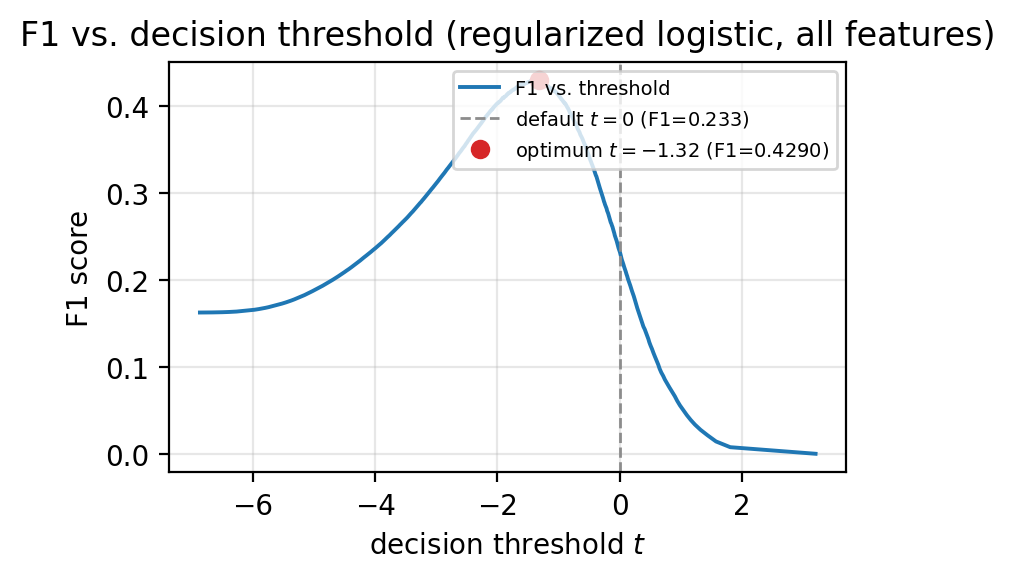
\includegraphics[width=\textwidth]{fig_threshold.png}
\captionof{figure}{F1 score of regularized logistic regression for different thresholds.}
\label{fig:threshold}
\end{minipage}

Table~\ref{tab:models} shows the results. The boosted trees are our best model with an F1 of 0.4357 ($\pm 0.003$ between folds), compared to 0.4290 for regularized logistic regression. The questions they use the most are general health, stroke, age, sex and diabetes. The linear models are all close to each other (0.419 to 0.429), except SGD, which is still far from converged after 20{,}000 steps of one sample.

The two things that changed the score the most were not the model itself. Using all the features instead of the 21 hand-picked ones raised F1 from 0.4125 to 0.4290, and choosing the threshold raised it from 0.233 (threshold 0.5) to 0.4290 (Figure~\ref{fig:threshold}).

We also tried a lot of things that did not help: new features (number of risk factors, number of chronic diseases, target encoding), a smaller learning rate, more bins, other models (additive models, random forests, nearest neighbours) and averaging several models. None of them changed the F1 by more than the difference between folds (about 0.003); the best average of several models reached 0.4373. All these models make the same mistakes, their predictions are 95--99\% correlated. With \texttt{HAREHAB1} the trees would reach 0.444, but only because of the leak.

\section{Conclusion}

Our final model is the boosted trees with a tuned threshold, with a cross-validated F1 of 0.4357. Most of the gain came from using all the data and from choosing the threshold, which agrees with \cite{domingos2012few}. Since very different methods all end up around 0.436, we think this is close to the limit of what these survey answers can predict. \texttt{python run.py} produces our submission and \texttt{python run\_linear.py} the results of the linear models.

\bibliographystyle{unsrt}
\small
\bibliography{literature}

\end{document}
